%%%%%%%%%%%%%%%%%%%%%%%%%%%%%%%%%%%%%%%%%%%%%%%%%%%%%%%%%%%%%%%%%%%%%%%%%%%%%%%%
%2345678901234567890123456789012345678901234567890123456789012345678901234567890
%        1         2         3         4         5         6         7         8

\documentclass[letterpaper, 10 pt, conference]{ieeeconf}  % Comment this line out
                                                          % if you need a4paper
%\documentclass[a4paper, 10pt, conference]{ieeeconf}      % Use this line for a4
                                                          % paper
\usepackage{hyperref}
\usepackage{url}
\usepackage{appendix}
\usepackage{amsmath}
\usepackage{algorithm}
\usepackage{amssymb}
\usepackage[noend]{algpseudocode}
\usepackage{graphicx}
\usepackage{subcaption}
\usepackage{wrapfig}
\IEEEoverridecommandlockouts                              % This command is only
                                                          % needed if you want to
                                                          % use the \thanks command
\overrideIEEEmargins
% See the \addtolength command later in the file to balance the column lengths
% on the last page of the document



% The following packages can be found on http:\\www.ctan.org
%\usepackage{graphics} % for pdf, bitmapped graphics files
%\usepackage{epsfig} % for postscript graphics files
%\usepackage{mathptmx} % assumes new font selection scheme installed
%\usepackage{times} % assumes new font selection scheme installed
%\usepackage{amsmath} % assumes amsmath package installed
%\usepackage{amssymb}  % assumes amsmath package installed

\title{\LARGE \bf
Bokeh Effect   
}


\author{ \parbox{2 in}{\centering  Harshal Mittal\\
    Dept. of Electronics Engg.\\
    IIT Roorkee\\    
   16116020 \\
        {\tt\small hmittal@ec.iitr.ac.in}}
        \hspace*{ 0.5 in}
        \parbox{2 in}{\centering Harshit Bansal\\
        Dept. of Electronics Engg.\\
    IIT Roorkee\\    
   16116021 \\
        {\tt\small hbansal@ec.iitr.ac.in}}
        \hspace*{ 0.5 in}
        \parbox{2 in}{\centering Shubham Maheshwari \\
        Dept. of Electronics Engg.\\
     IIT Roorkee\\    
16116065\\
        {\tt\small smaheshwari@ec.iitr.ac.in}
        \hspace*{ 0.5 in}}
}


\begin{document}



\maketitle
\thispagestyle{empty}
\pagestyle{empty}





%%%%%%%%%%%%%%%%%%%%%%%%%%%%%%%%%%%%%%%%%%%%%%%%%%%%%%%%%%%%%%%%%%%%%%%%%%%%%%%%
\begin{abstract}

In this project, we aim to produce a Bokeh effect from a single image. The main principle behind this effect is depth mapping. Depth mapping is a prediction of depth at each point in the image. Thus, given a depth mapping, and a pre-defined threshold, we can approximately classify the points into foreground and background. The background points would be applied a Gaussian kernel, producing a blur effect, while the foreground mask can be simply applied to the original image. The two would then be concatenated to produce the final Bokeh image. Also, the depth map of an image is directly related to its defocus map, given the camera parameters. However, due to the focal plane ambiguity, it is generally assumed that all de-focussed pixels lie on one side of the focal plane and the focussed on the other side, producing a rough depth map. Thus the problem reduces to that of defocus map estimation, which has been extensively discussed in the past.

\end{abstract}


%%%%%%%%%%%%%%%%%%%%%%%%%%%%%%%%%%%%%%%%%%%%%%%%%%%%%%%%%%%%%%%%%%%%%%%%%%%%%%%%
\section{INTRODUCTION}
Defocus blur estimation plays an important role in many computer
vision and computer graphics applications including depth estimation, image deblurring and refocusing. Previously, the problem has been tackled by taking two images at varying depths or through the use of portrait lenses. However, recent attention has been shifted towards depth estimation from a single image taken from an ordinary camera. The project aims to utilize defocus blur estimation to produce a Bokeh effect from a single image. This is done by segmenting the image into two parts: foreground and background based on the value of the defocus blur, and further applying a Gaussian kernel to the background. Defocus blur is estimated from the ratio of the magnitude of the gradients of the original and the re-blurred image. 
\begin{figure}[h]
\begin{subfigure}{0.5\textwidth}
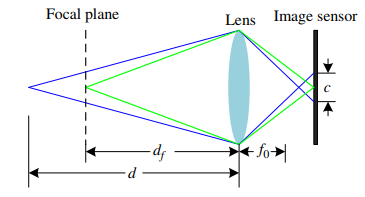
\includegraphics[width=1\linewidth, height=5cm]{lens.png}
\label{fig:subim13}
\end{subfigure}
\caption{Focus and defocus for thin lens model.}
\label{fig:image23}
\end{figure}

The overall flow of the report can be described as follows: In section 2, the defocus model is introduced. In section 3, the overall procedure of the algorithm is explained followed by the results in section 4. Finally, the project report ends with some limitations of the program and the conclusion.  
                              
\section{DEFOCUS MODEL}
When an image is taken from a camera, only the points lying on the focal plane of the camera would be on focus. The rest of the points would have more than one mapping on the screen producing a blur effect.

Assuming that the focus and defocus obey the thin lens model, when an object is placed at distance d\textsubscript{f} from the lens, all the rays emerging from it would be converged at a single point on the sensor by the lens, thus producing a sharp image. While if the object is at a distance d from the lens, the rays produced by it will reach multiple sensor points on passing through the lens, and would result in a blurred image. This is shown in Fig 1. 
The blur pattern on the sensor plane depends on the lens aperture, and is called the ‘Circle of Confusion’ (CoC), whose diameter can be approximated as :
$$
c=\frac{|d-d\textsubscript{f}|}{d}\frac{f\textsubscript{o}^2}{N(d-d\textsubscript{f})}\eqno{(1)}
$$

where $\sigma$  = kc measures the defocus blur amount at any point and is proportional to the diameter of CoC. It is further explained in the next section.
\begin{figure*}[t]
\centering
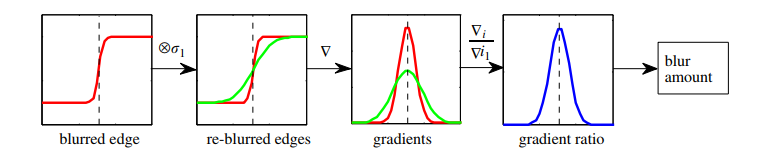
\includegraphics[width=15cm, height=2.5cm]{edge.png}
\label{fig:subim13}
\caption{The overview of our blur estimation approach: here,  $\ast$ and $\nabla$ are the convolution and gradient operators, respectively. The black dash line denotes the edge
location at x=0.}
\end{figure*}
\section{PROCEDURE}
\subsection{Extracting the sparse defocus map}
The defocus blur is taken only at the edges present in the image, which can be represented ideally as:
$$
f(x)=Au(x)+B\eqno{(2)}
$$
The defocus blur can be understood as applying the convolution operator on the edge and the PSF (Point Spread Function), where the PSF is approximated by a Gaussian Function g(x,$\sigma$ ) The $\sigma$ here is the measure of the defocus blur amount, and $\sigma$ = kc (relating it to the CoC as mentioned previously). The blurred edge can then be written as : 
$$
i(x) = f(x) \ast g(x, \sigma)\eqno{(3)}
$$
We estimate the defocus blur (estimated only at edges) amount by first calculating the ratio between the gradient magnitudes in the original image and the re-blurred image at the edges as shown in Fig 2.
We call this ratio as {R} and it would be higher at the edges compared to other points in the image, as expected. This is because the effect of blurring would be more pronounced at the edges compared to other image points, as the other points were already a bit soft and not so sharp, while the edges were smudge-free in the original image. This can also be proved mathematically as follows :
\\

\hspace*{1ex}$\nabla i_1(x) = \nabla(i(x) \ast g(x, \sigma_0))$
\hspace*{14ex}(4)
\hspace*{15ex}$=\nabla((Au(x)+B) \ast g(x, \sigma) \ast g(x, \sigma_0))$

 
\hspace*{13ex}$= \frac{A}{\sqrt{2 \pi (\sigma^2 + \sigma_0^2)}}\exp(-\frac{x^2}{2(\sigma^2 + \sigma_0^2)}))$
\\

Here, $\sigma_0$ is the standard deviation of the re-blur Gaussian kernel.


The ratio of the gradient magnitudes between the original and re-blurred image is calculated as:

$$
\frac{|\nabla i(x)|}{|\nabla i_1(x)|} = \sqrt{\frac{\sigma^2 + \sigma_0^2}{\sigma^2}} \exp(-(\frac{x^2}{2 \sigma^2} - \frac{x^2}{2(\sigma^2 + \sigma_0^2)})) \eqno{(5)}
$$

The ratio is maximum at the edge location(x = 0) and the maximun value is given by : 

$$
 R = \frac{|\nabla i(0)|}{|\nabla i_1(0)|} = \sqrt{\frac{\sigma^2 + \sigma_0^2}{\sigma^2}} \eqno{(6)}
$$


We can see that the maximum of the gradient magnitude ratio R eliminates the effect of edge amplitude A, and depends only on original image blur $\sigma$ and the re-blur amount $\sigma_0$.
\\

This was the case for 1D, blur estimation for 2D images is done along the same lines. A 2D isotropic Gaussian kernel is used for re-blurring and the gradient magnitude can be calculated as:

$$
||\nabla i(x, y) || = \sqrt{\nabla i_x^2 + \nabla i_y^2} \eqno{(7)}
$$


Once R is obtained, the unknown blur amount $\sigma$ of the original image can be obtained as:
$$
\sigma =\frac{1}{\sqrt{R^2-1}}\sigma_0\eqno{(8)}
$$
In our implementation, we found out the re-blur amount $\sigma_0$ to be 1 by trying out a few different values, as $\sigma_0$ = 1 was giving acceptable results.
As mentioned, the defocus blur is estimated only at edges. So $\sigma$ at other points in the image is made 0 by first using Canny-Edge detection to obtain the edge points,  and then applying a mask (comprising of non-edge points) to the defocus blur map to set the values to 0.
This sparse defocus map (or sparse depth map) is denoted by \^d(x). To remove the inaccuracies present in it due to weak or noisy edges, a Joint Bilateral Filter (JBF) is applied to refine the sparse defocus map.

\subsection{Bilateral Filtering}
The defocus blur can be understood as applying the convolution operator on the edge and the PSF (Point Spread Function), where the PSF is approximated by a Gaussian Function
The sparse defocus blur map, which has been obtained at edge locations may contain some inaccuracies due to the quantization error at weak edges and noise or soft shadows in the image. Thus, joint bilateral filtering is applied to the sparse depth map to correct the wrong blur estimates. It thereby avoids the propagation of the errors in the defocus map interpolation as explained in the next section.

\subsection{Defocus Map Interpolation}

The defocus blur estimation method produces a sparse depth map which needs to be propagated to the full image to obtain the full depth map. Matting Laplacian, an edge-aware interpolation method is used to do the defocus map interpolation. It seeks to produce a depth map close to the sparse depth map and also aligning the discontinuities with the image edges. 
Overall, it aims to minimize the following loss function:
$$
E(d)=d\textsuperscript{T}Ld+\lambda(d-\^d)\textsuperscript{T}D(d-\^d) \eqno{(9)}
$$

where \textit{\^d} and \textit{d} are the vector forms of the sparse defocus map and the full defocus map respectively.\textit{ L} is the matting Laplacian matrix and \textit{ D} is a diagonal matrix whose element \textit{D\textsubscript{ii}}  is 1 if pixel \textit{i} is at the edge location, and 0 otherwise. 
The optimal {d} can be obtained by solving the following sparse
linear system:
$$
(L+\lambda D)d=\lambda D\^d\eqno{(10)}
$$

\begin{figure*}[t]
\centering
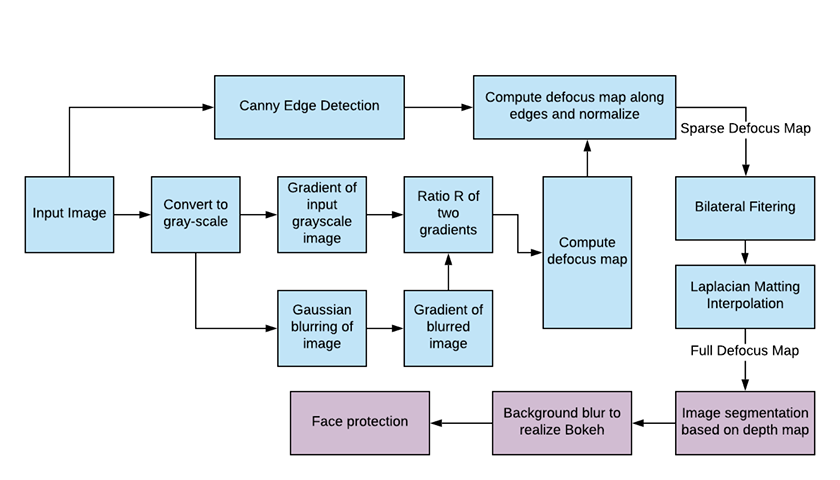
\includegraphics[width=15cm, height=7cm]{graph.png}
\label{fig:subim14}
\caption{Algorithm Flowchart.}
\end{figure*}
\subsection{Bokeh Effect}

To achieve Bokeh effect after the full depth map estimation, the image can be segmented into two segmentations i.e., foreground and background. This would be done by deciding an appropriate threshold and considering all the points with their depth/defocus blur below the threshold as a part of the foreground and the remaining as background. Thus, the bit masks of these segmentations would be obtained. The bit mask of the foreground would be applied on the original image and the bit mask of the background would be applied on the blurred image which is obtained by applying a Gaussian kernel to the original image. Finally, both images are combined to produce the final image with the Bokeh effect. Due to the imperfect segmentations, some parts of the face like eyebrow, hair are usually blurred as they are segmented into the background. To resolve this problem, face detection can be used to avoid blurring of the face. If the face is detected on the original image using Matlab Computer Vision Toolbox and the average depth (or defocus blur) of the face region is small, no blur would be applied regardless of the result. The position and size of the rectangular box, returned by face detection algorithm of Matlab Computer Vision Toolbox, need to be adjusted as this box region only covers the face but excludes the hair.

The flowchart of the overall algorithm is presented in Figure 3.

\begin{figure*}[h]
\centering
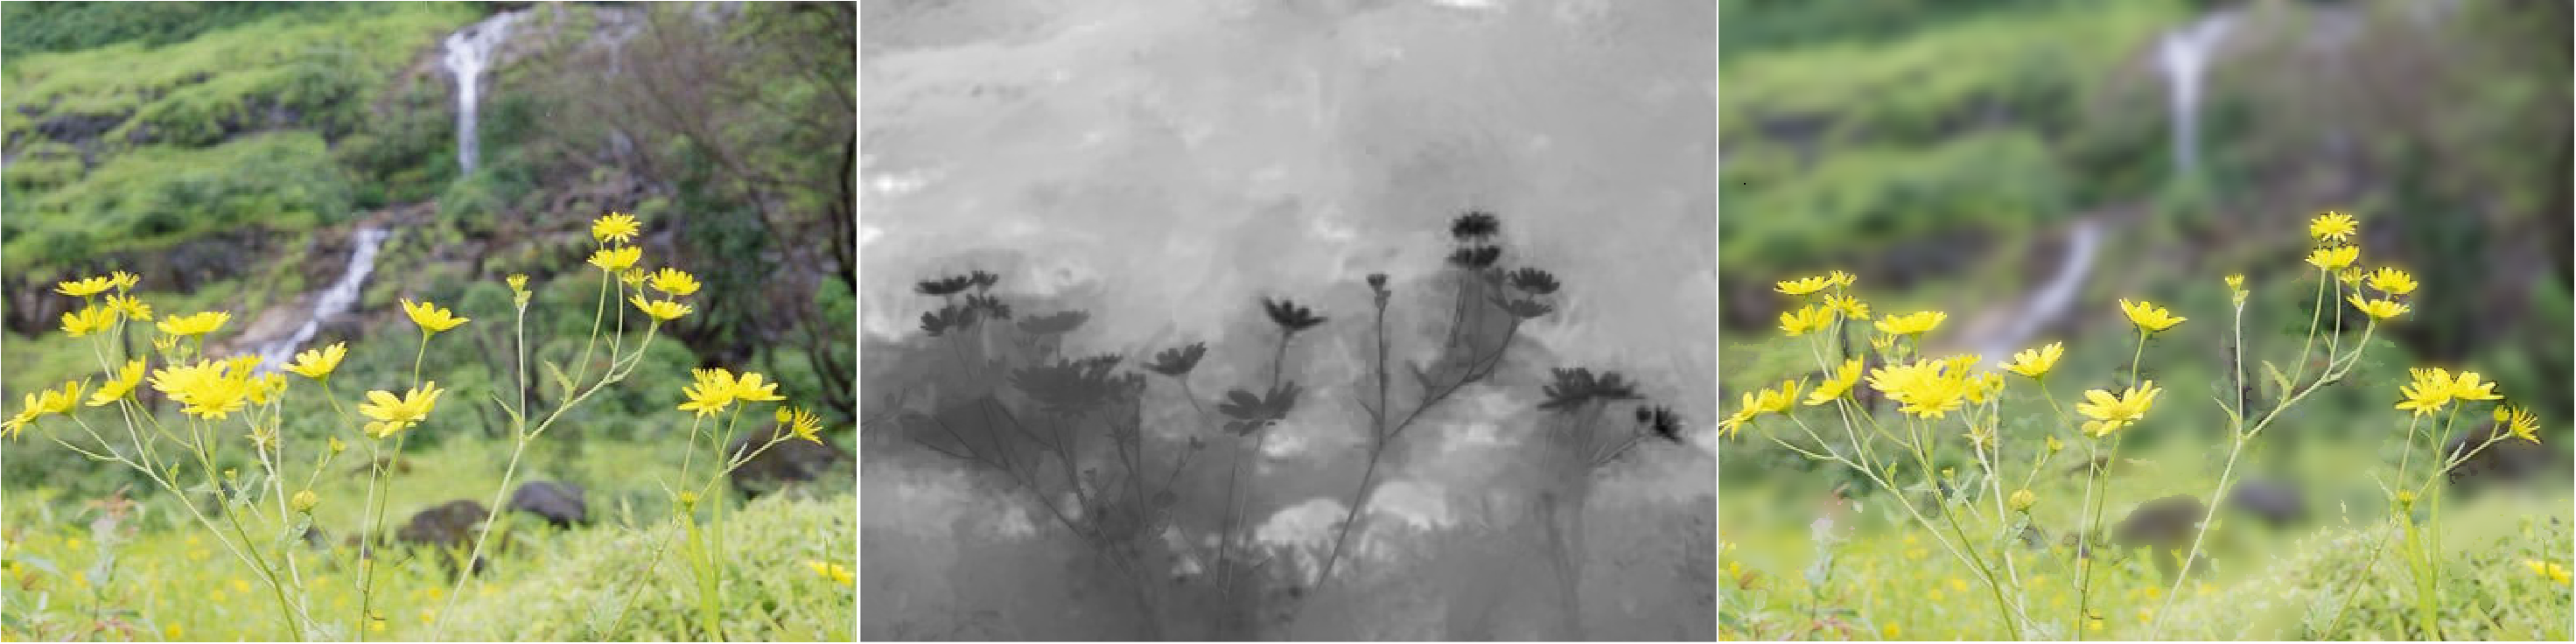
\includegraphics[width=16cm, height=5cm]{out1.png}
\label{fig:subim14}
\caption{Left: Original Image, Center: Extracted full Defocus map, Right: Resultant image after Bokeh Effect.}
\end{figure*}

\begin{figure*}[h]
\centering
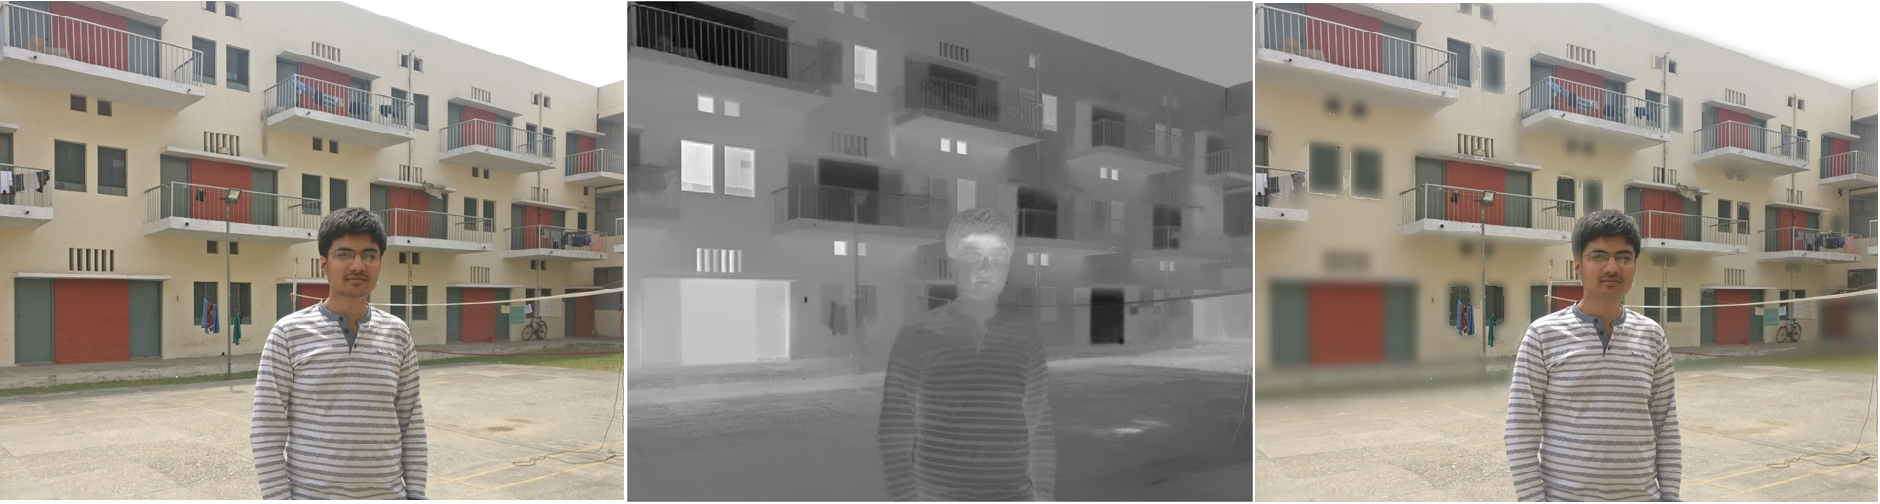
\includegraphics[width=16cm, height=5cm]{out.png}
\label{fig:subim14}
\caption{Left: Original Image, Center: Extracted full Defocus map, Right: Resultant image after Bokeh Effect.}
\end{figure*}
\begin{figure*}[h]
\centering
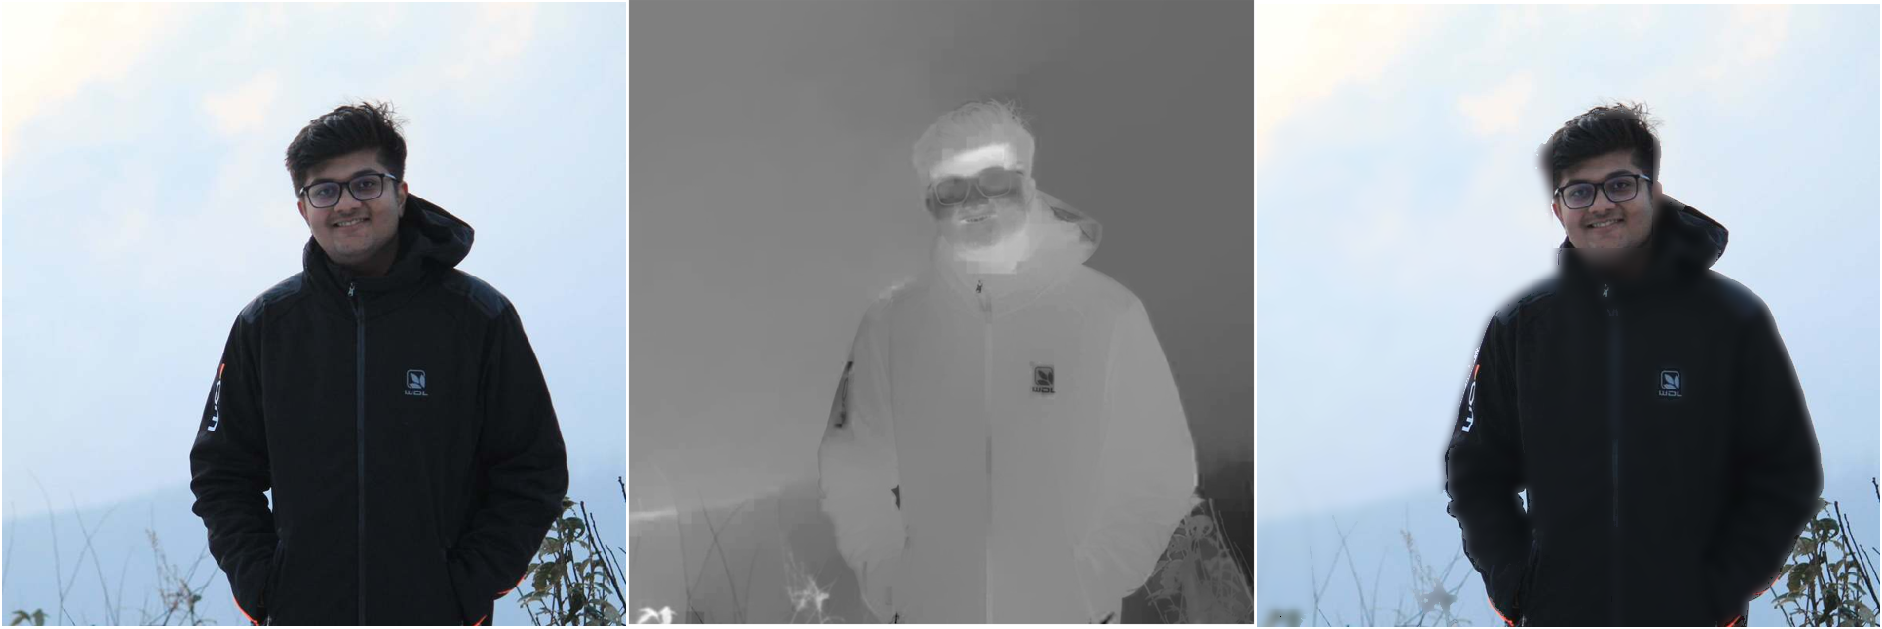
\includegraphics[width=16cm, height=5cm]{out2.png}
\label{fig:subim14}
\caption{Left: Original Image, Center: Extracted full Defocus map, Right: Resultant image after Bokeh Effect.}
\end{figure*}
\section{RESULT}

The results are good when sharp edges are present for the foreground objects and some amount of defocus blur is present for the background objects. This is because the algorithm for the estimation of the sparse defocus map considers the ratio of the gradients of the original and the blurred image at the edges. A blurred background would have a relatively smaller gradient ratio, thus assigning it a high defocus blur. Due to the same reason, sharp edges would have a higher gradient ratio and thus a small defocus blur. The joint bilateral filtering algorithm also results in a more continuous and accurate sparse defocus map. The face detection algorithm further improves the results whenever the algorithm blurs the facial parts. 

The results of the algorithm on some images are shown in Figures 4, 5, and 6. As can be seen in Figure 4, the image consists of flowers in the foreground having sharp edges and a relatively blurred background. The algorithm successfully segments the foreground from the background and generates appreciable results. In Figure 5, the face of the person had some amount of blur, which was rectified by the face protection part. Also, an instance of the failure of the algorithm is depicted in Figure 6. Here, the image has a bigger depth map with background having no defocus blur. Thus, the algorithm fails to blur the background and incorrectly blurs the clothes of the person.      



\section{LIMITATIONS AND FUTURE WORK}

Defocus blur is more pronounced in cameras which have a shallow depth of field and is less pronounced in a camera with a larger depth of field. Generally, cheaper cameras have a larger depth of field whereas expensive cameras have a shallow depth of field. Hence this method would generate a poor result whenever the background of the image has less defocus blur. Another limitation is the non-smooth transition between foreground and background on the output image. This happens due to the abrupt shift in the levels of blurring between the two different segmentations. This can be partially resolved by implementing a more gradual and continuous Gaussian kernel along the points where the two segmentations are concatenated and we also intend to do as future work.


%%%%%%%%%%%%%%%%%%%%%%%%%%%%%%%%%%%%%%%%%%%%%%%%%%%%%%%%%%%%%%%%%%%%%%%%%%%%%%%%
\break
\break
\break
\break
\break
\section*{ACKNOWLEDGMENT}

We would like to thank Professor Saumik Bhattacharya for providing us the opportunity to work on this project and guiding us throughout. We learnt a lot during the entire period, which was a very indulging experience and would also prove to be helpful further.




%%%%%%%%%%%%%%%%%%%%%%%%%%%%%%%%%%%%%%%%%%%%%%%%%%%%%%%%%%%%%%%%%%%%%%%%%%%%%%%%

\begin{thebibliography}{99}

\bibitem{c1} X. Zhu, S Cohen, S Schiller, and P. Millanfar Estimating Spatially Varying Defocus Blur. IEEE Transactions on,
volume 22, pages 4879 – 4891, 2013.
\bibitem{c2} A. Chakrabarti, T. Zickler, and W. T. Freeman “Analyzing spatially varying blur" in Proc. IEEE CVPR, Jun.
2010,pp. 2512–2519.
\bibitem{c3} A. Levin, R. Fergus, F. Durand, and W. T. Freeman. Image and depth from a conventional camera with a coded
aperture. ACM Trans. Graphics, 2007.
\bibitem{c4} P. Favaro, S. Soatto, A geometric approach to shape from defocus, IEEE Trans.Pattern Anal. Mach. Intell. 27 (3) (2005) 406–417.
\bibitem{c5} A.P. Pentland, A new sense for depth of field, IEEE Trans. Pattern Anal. Mach. Intell. 9 (4) (1987) 523–531.


\end{thebibliography}

\end{document}
